\chapter*{Trabajo académico 12/03/2025}

\lstset{language=python}


% \note{Sé que un mi compañero prenguntó si podía escribir en inglés, y que está bien; hablo bastante bien español y habeis empezado pero Me resulta más confortable y natural escribir en inglés, y creo que sea mejor que confiar en ChatGPT (y similares) para la corrección de la traducción \smiley.}

\note{Sé que un mi compañero prenguntó si podía escribir en inglés, y que está bien; Hablo español bastante bien, pero me resulta más natural escribir en inglés; sin embargo, decidí escribir en español para practicar, con la ayuda de algunos traductores cuando era necesario. Si hay algo mal escrito o poco claro, estoy a disposición para cualquier aclaración.}

\section{Introducción}

He eligido el \textbf{dominio de emergencias} para mi trabajo. Resumiendo lo que está escrito en la tarea, en este dominio los puntos de interés son los siguientes:
\begin{itemize}
   \item Localización de las víctimas, ambulancias y hospitales.
   \item Asignación de ambulancias a las víctimas, teniendo en cuenta la gravedad de la emergencia.
   \item Minimización del tiempo de respuesta, como objetivo.
\end{itemize}

La version más basica del escenario incluye una sola víctima, en vez la version ampliada mas victímas.

\section{Implementación}

\subsection{Representación del estado}
El estado se representa con alguno diccionarios, uno para cada entidad:
\begin{lstlisting}
   state1.ambulances = [ {'label': 'A1', 'cap': 10, 'loc': 'El Carmen'},...
   state1.victims = [ {'name': 'Carlos', 'sev': 5, 'loc': 'El Carmen'},...
   state1.hospitals = [ {'name': 'H1', 'loc': 'Hospital La Fe'},...
\end{lstlisting}
En cada entrada del diccionario se encuentran propiedades de la entidad como la posición, el nombre y la gravedad.

Hay tambien una función para trazar el grafo de las localidades, que son barrios de la ciudad de Valencia.
\note{No es perfecta, pero fue útil para analizar el escenario}
\begin{figure}[htbp]
   \centering
   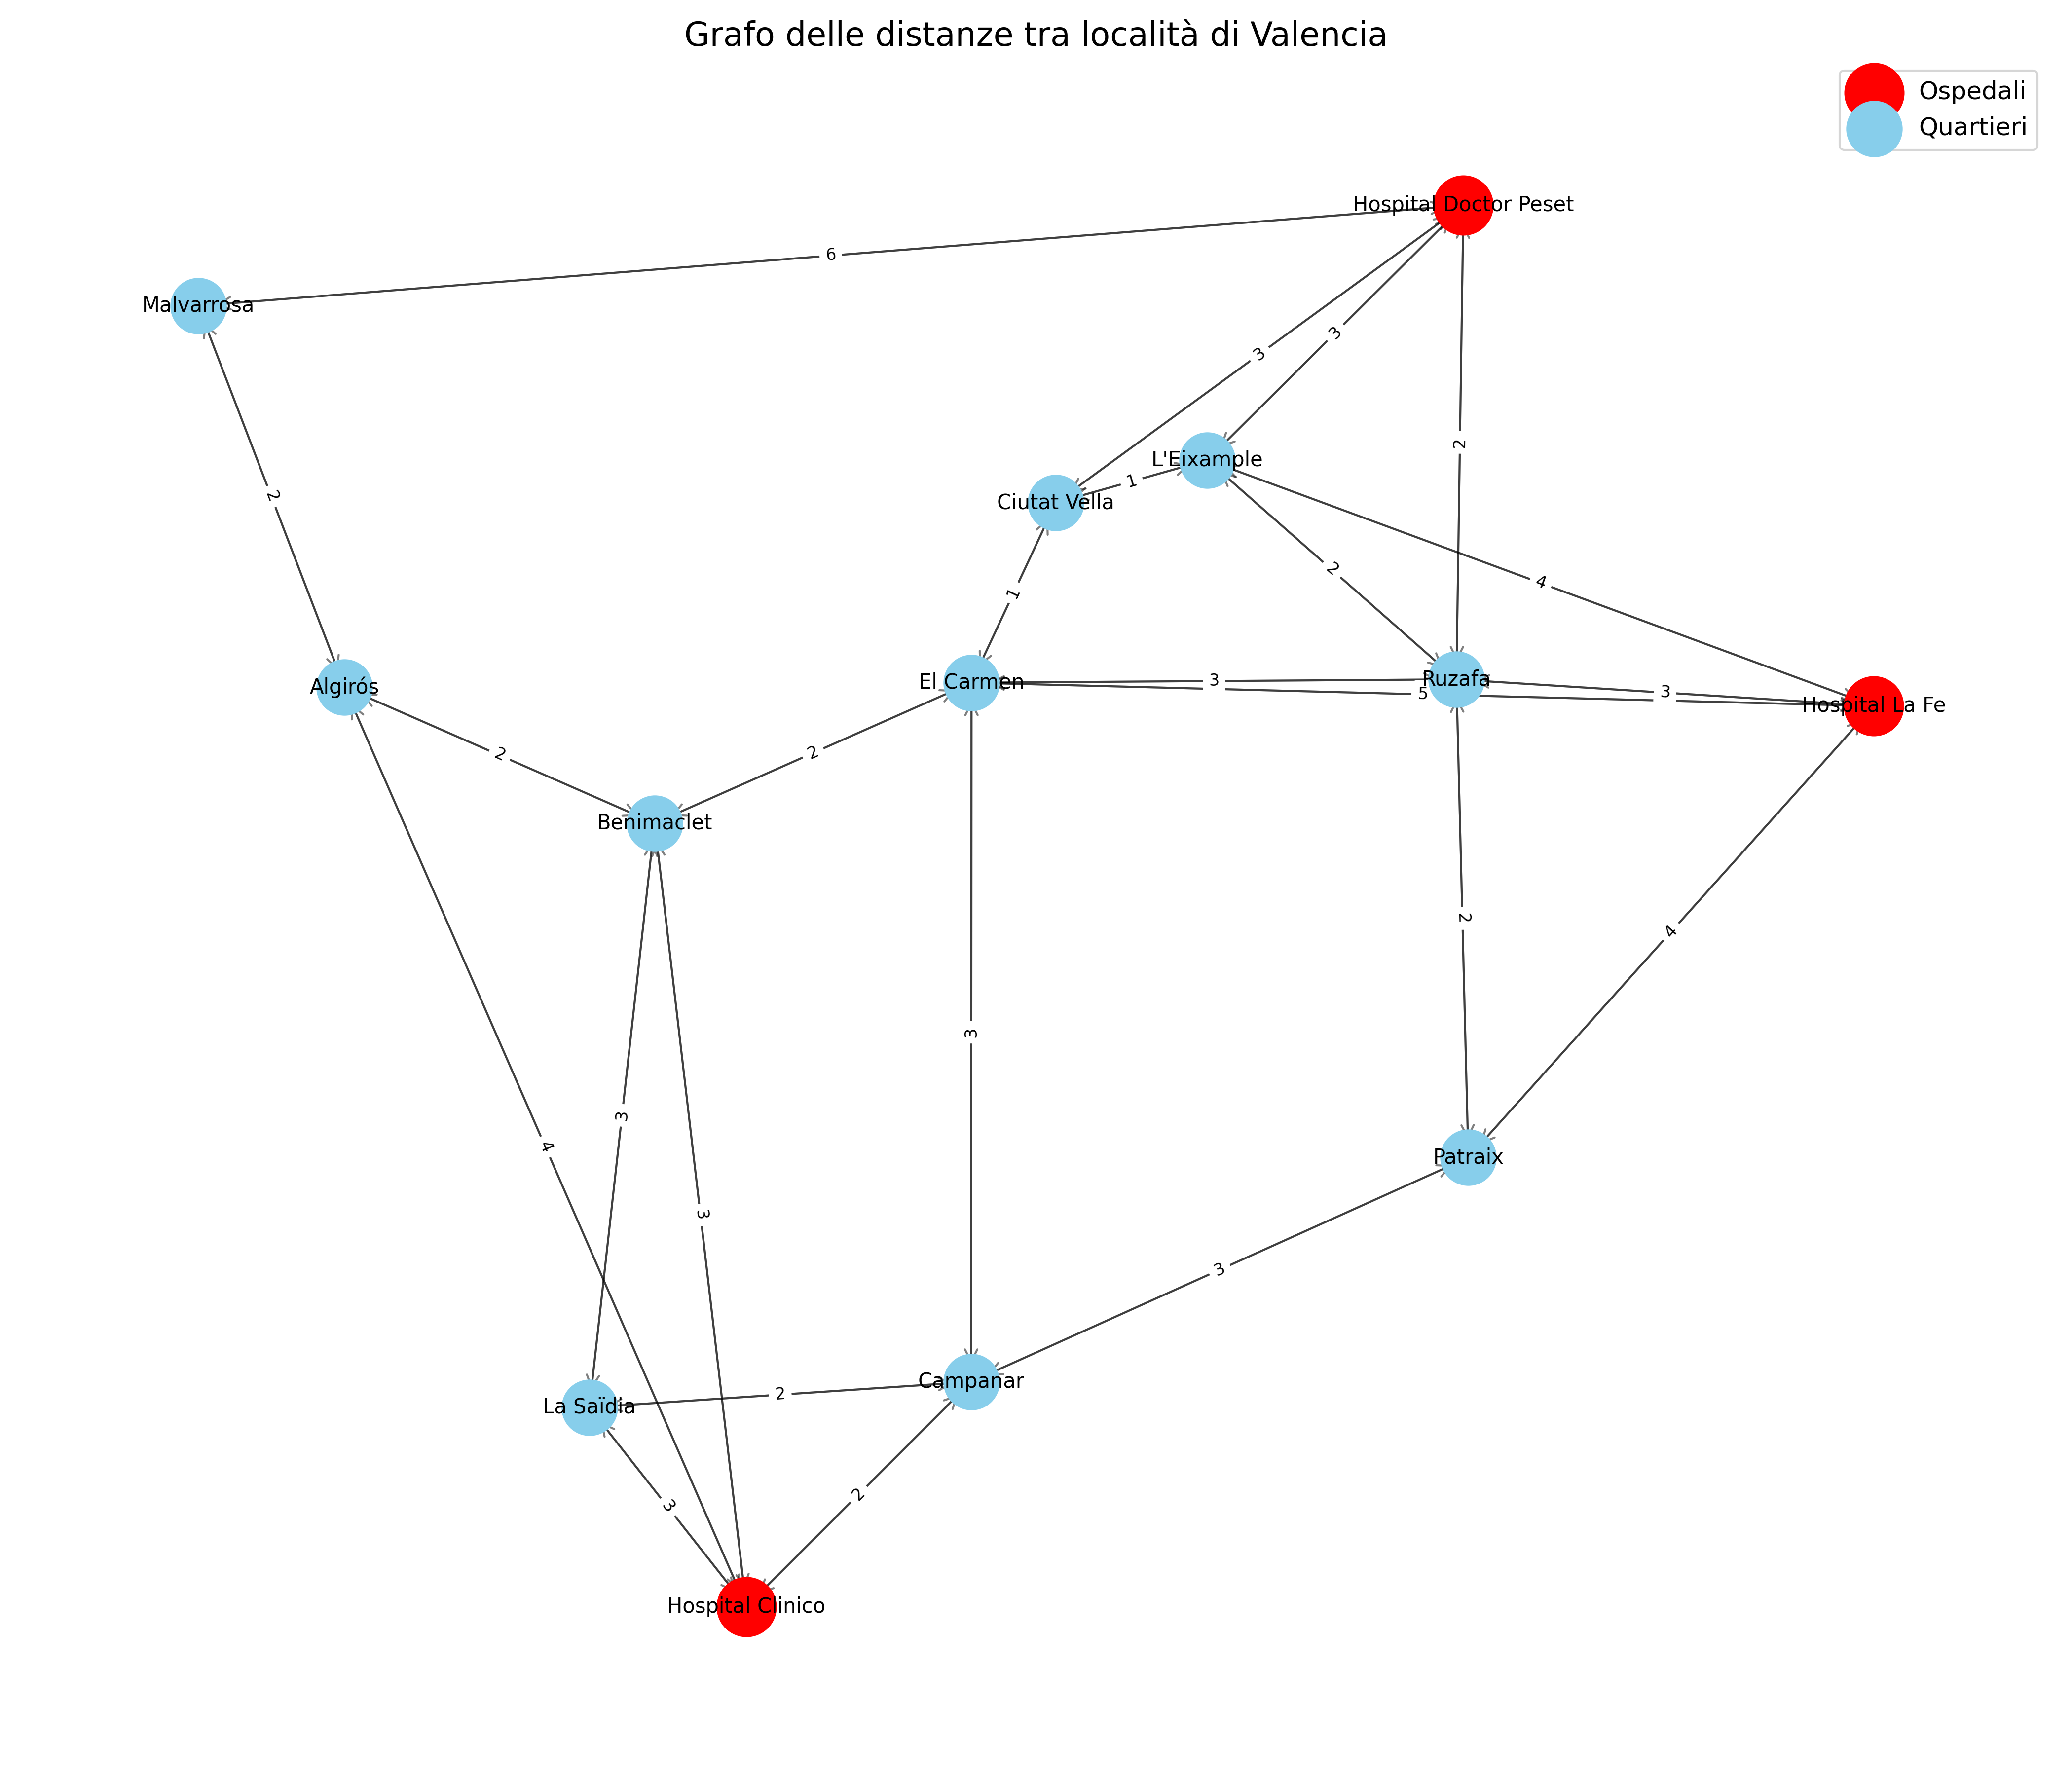
\includegraphics{images/06/valencia_graph.png}
   \caption{Grafo de las localidades de Valencia}
   \label{fig:06/valencia_graph}
\end{figure}

\subsection{Operadores}

\subsection{Métodos}

La manera más intuitiva y clara de implementar la gestión de multiple victímas es de llamar recursivamente el método de búsqueda para cada victima.
\begin{lstlisting}
   def method_deliver_all(state):
   if not state.victims:
       return []  # Base case: no more victims to deliver.
   
   # Take the first victim in the list.
   victim = state.victims[0]
   return [('deliver_victim', victim, 'H1'),
           ('op_remove_victim', victim['name']),
           ('deliver_all',)]

\end{lstlisting}

Sin embargo, esta Implementación no garantiza la minimización del tiempo total de respuesta, porque el método no tiene cuenta que la ambulancia que lleva la primera victima puede ser la más cercana a la segunda victima.
Considere este escenario:
$v_1$ està en $l_1$, $v_2$ està en $l_2$ y $a_1$ està en $l_2$. El hospital 

